%% PEARC '26 camera-ready: VGAC paper
%% DOI 10.1145/3785462.3815816
\documentclass[sigconf]{acmart}

%% --------- ACM rights/permissions/conference (from acceptance email) ---------
\copyrightyear{2026}
\acmYear{2026}
\setcopyright{cc}
\setcctype{by}
\acmConference[PEARC '26]{Practice and Experience in Advanced Research Computing}{July 26--30, 2026}{Minneapolis, MN, USA}
\acmBooktitle{Practice and Experience in Advanced Research Computing (PEARC '26), July 26--30, 2026, Minneapolis, MN, USA}
\acmDOI{10.1145/3785462.3815816}
\acmISBN{979-8-4007-2377-3/2026/07}

%% --------- Packages (TAPS-accepted set) ---------
\usepackage{booktabs}
\usepackage{amsmath}
\usepackage{xcolor}
\usepackage{microtype}
\usepackage{graphicx}

%% Figures live in ../figures/ relative to tex/; for the TAPS upload the
%% figure files are shipped alongside the .tex so this also resolves to ./.
\graphicspath{{../figures/}{./figures/}{./}}

%% Allow modest extra inter-word stretch to absorb tight inline texttt{} runs
%% in narrow ACM sigconf columns without any explicit hyphenation overrides.
\emergencystretch=2em

%% --------- CCS / keywords plumbing handled by acmart ---------

\begin{document}

\title{VGAC: A Full-Stack GPU Cluster Observability Platform with Calibration-Gated Predictive Intelligence}

\author{Andrew Espira}
\orcid{0009-0002-9196-8094}
\affiliation{%
  \institution{Saint Peter's University}
  \department{Department of Data Science}
  \city{Jersey City}
  \state{NJ}
  \country{USA}
}
\email{aespira@saintpeters.edu}

\author{Sharath Kumar}
\affiliation{%
  \institution{Saint Peter's University}
  \department{Department of Data Science}
  \city{Jersey City}
  \state{NJ}
  \country{USA}
}
\email{skumar@saintpeters.edu}

\renewcommand{\shortauthors}{Espira and Kumar}

\begin{abstract}
Calibrated queue-delay predictions are useful only if they translate into scheduling decisions with known operating characteristics. We present VGAC, a full-stack GPU cluster observability platform with calibration-gated predictive intelligence: each predictive intervention is permitted only when the underlying probability is calibrated well enough to support it. The contribution has three parts. (1) A graduated intervention framework with four tiers---Annotate, Warn, Suggest, Gate---each carrying an explicit calibration prerequisite (Expected Calibration Error $\le 0.10$ for Annotate down to ECE $\le 0.03$ for Gate) and a tier-specific probability threshold $\varepsilon_a$ in the rule ``apply action $a$ if $\hat{p} \ge \varepsilon_a$.'' (2) A submit-time queue-state capture methodology that corrects an inverted feature correlation, taking Pearson $r$ from $-0.27$ under naive 30\,s polling to $+0.44$ under submit-time capture, and so establishes correct measurement as a prerequisite for correct decision rules. (3) An empirical floor-to-ceiling validation on an Amazon EKS GPU cluster: a 2-feature ``floor'' model qualifies for Annotate and is marginal for Warn (AUROC 0.756, ECE 0.077), while the 17+\,feature production VGAC model achieves ECE 0.005 and qualifies for all four tiers including autonomous admission gating. The framework is realized in production-grade Kubernetes admission webhooks and Slurm \texttt{job\_submit} hooks that re-evaluate tier qualification at serve time so degraded models automatically reduce their action scope.
\end{abstract}

\begin{CCSXML}
<ccs2012>
<concept>
<concept_id>10010520.10010553.10010554</concept_id>
<concept_desc>Computer systems organization~Cloud computing</concept_desc>
<concept_significance>500</concept_significance>
</concept>
<concept>
<concept_id>10010147.10010257.10010293.10010294</concept_id>
<concept_desc>Computing methodologies~Supervised learning by classification</concept_desc>
<concept_significance>300</concept_significance>
</concept>
</ccs2012>
\end{CCSXML}
\ccsdesc[500]{Computer systems organization~Cloud computing}
\ccsdesc[300]{Computing methodologies~Supervised learning by classification}

\keywords{GPU cluster observability, calibration-gated decisions, Expected Calibration Error, graduated intervention, submit-time capture, Kubernetes admission webhook, Slurm job\_submit plugin}

\maketitle

\section{Introduction}
\label{sec:intro}
A growing body of work has demonstrated that queue-delay predictions can be made calibrated---that $\hat{p}=P(\text{delay} > T)$ can be made to match realized frequencies~\cite{guo2017calibration}. A companion paper~\cite{espira2026reliability} defines the service-level indicators (SLIs) and service-level objectives (SLOs) for monitoring this calibration in production. But a calibrated probability alone does not tell a scheduler what to do. The missing piece is a decision-theoretic bridge: formal rules that translate $\hat{p}$ into actions, with explicit prerequisites on how calibrated $\hat{p}$ must be for each action to be trustworthy.

Current GPU schedulers~\cite{borg,firmament} are reactive: they queue a job and observe what happens. Predictive systems can improve this by providing risk estimates at submit time. But the operational question remains: given $\hat{p}=0.73$ for a submitted job, should the system (a) do nothing, (b) annotate the job with a warning, (c) suggest rescheduling, or (d) gate the submission pending confirmation?

The answer depends on two factors: the severity of the action and the trustworthiness of $\hat{p}$. A low-stakes annotation can tolerate moderate miscalibration; an admission gate that blocks submissions must be backed by highly calibrated probabilities, or users will lose trust and override the system. We formalize this intuition into a graduated intervention framework and instantiate it in VGAC, a full-stack observability platform whose predictive intelligence is \emph{calibration-gated}: each tier of intervention is permitted only when the underlying model has earned the calibration quality the action requires.

\subsection{Contributions}
We contribute: (1) a decision-theoretic framework with four intervention tiers, each paired with a formal calibration prerequisite; (2) the decision rule ``apply action $a$ if $P(\text{delay} > T) \ge \varepsilon_a$'' with tier-specific thresholds; (3) a submit-time queue-state capture methodology that corrects an inverted feature correlation ($r=-0.27 \to r=+0.44$); (4) an honest tier-qualification analysis showing the 2-feature floor model (ECE 0.077) qualifies for Annotate but not Suggest/Gate, while the 17+\,feature production VGAC model (ECE 0.005) qualifies for all four tiers; and (5) reference implementations for Kubernetes mutating admission webhooks and Slurm \texttt{job\_submit} plugins that enforce tier qualification dynamically at serve time.

\section{Background}
\subsection{From Prediction to Decision}
Prior work on cluster-scheduling prediction~\cite{decima} focuses on placement optimization; our focus is on the human-system interface at submit time. Calibration methods~\cite{guo2017calibration,platt1999} ensure $\hat{p}$ matches reality; we address what to do with a calibrated $\hat{p}$.

\subsection{Decision Theory for Classification}
In medical diagnosis, a calibrated probability $P(\text{disease})$ is combined with a cost matrix to determine whether to treat~\cite{elkan2001}. We apply the same logic to scheduling: each tier has an action cost (from zero for annotation to high for submission gating), and the calibration prerequisite ensures the expected cost of acting on a miscalibrated $\hat{p}$ remains below an acceptable threshold.

\section{Graduated Intervention Framework}
\label{sec:framework}

\subsection{Decision Rule}
Let $\hat{p}_j = P(\text{delay}_j > T)$ be the calibrated probability that job $j$ will violate its SLO. The system applies action $a$ if
\begin{equation}
\hat{p}_j \;\ge\; \varepsilon_a,
\label{eq:rule}
\end{equation}
where $\varepsilon_a$ is a tier-specific probability threshold.

\subsection{Intervention Tiers}
Table~\ref{tab:tiers} enumerates the four tiers, their decision thresholds, and their calibration prerequisites.

\begin{table}[t]
\centering
\caption{Graduated intervention tiers with calibration prerequisites.}
\label{tab:tiers}
\small
\begin{tabular}{@{}llrr@{}}
\toprule
\textbf{Tier} & \textbf{Action} & \textbf{$\varepsilon_a$} & \textbf{ECE Prereq.} \\
\midrule
1: Annotate & Add risk label          & 0.3 & $\le 0.10$ \\
2: Warn     & Notify user             & 0.5 & $\le 0.07$ \\
3: Suggest  & Recommend reschedule    & 0.7 & $\le 0.05$ \\
4: Gate     & Require confirmation    & 0.9 & $\le 0.03$ \\
\bottomrule
\end{tabular}
\end{table}

The prerequisite column encodes the key insight: higher-stakes actions demand better-calibrated models. Tier~1 (Annotate) is informational---10\,pp of miscalibration is still directionally correct (ECE $\le 0.10$). Tier~2 (Warn) interrupts the user's workflow, so excessive false warnings erode trust (ECE $\le 0.07$). Tier~3 (Suggest) implies high confidence in delay occurrence (ECE $\le 0.05$). Tier~4 (Gate) blocks submissions---users abandon systems where gating is wrong more than $\sim 3\%$ of the time (ECE $\le 0.03$).

\subsection{Graceful Degradation}
When model quality degrades (ECE rises above a tier's prerequisite), the system automatically disables that tier and falls back to the highest tier still qualified. A model with ECE $=0.06$ enables Tiers 1--2 but disables Tiers 3--4. This provides safety without total system shutdown and creates a natural feedback loop: degradation is visible in reduced functionality, motivating recalibration.

\section{Submit-Time Capture Methodology}
\label{sec:submit-time}
Correct decision rules require correct input features. We discovered a critical measurement error: periodic queue snapshots produce inverted feature correlations.

\subsection{The Snapshot Timing Problem}
Initial data collection captured queue state by periodic polling at 30\,s intervals. Analysis revealed Pearson $r=-0.27$ between \texttt{pending\_at\_submit} and observed wait time: more pending jobs predicted shorter waits. The root cause is straightforward: queue state was captured at observation time, not at the moment of job submission. By the time a job is observed as ``Pending,'' the queue has already drained.

\subsection{Corrected Collection}
We redesigned the collector to capture queue state at the exact moment of job submission: poll every 5\,s, detect phase transitions (Pending~$\to$~Running~$\to$~Succeeded), and record queue state at each transition. Table~\ref{tab:correlation} reports the corrected correlation.

\begin{table}[t]
\centering
\caption{Feature correlation: snapshot vs.\ submit-time capture.}
\label{tab:correlation}
\small
\begin{tabular}{@{}llp{0.3\linewidth}@{}}
\toprule
\textbf{Method} & \textbf{Correlation} & \textbf{Interpretation} \\
\midrule
Periodic snapshot (30\,s)   & $r=-0.27$ & Inverted (wrong) \\
Submit-time capture (5\,s)  & $r=+0.44$ & Correct \\
\bottomrule
\end{tabular}
\end{table}

\begin{figure}[t]
\centering
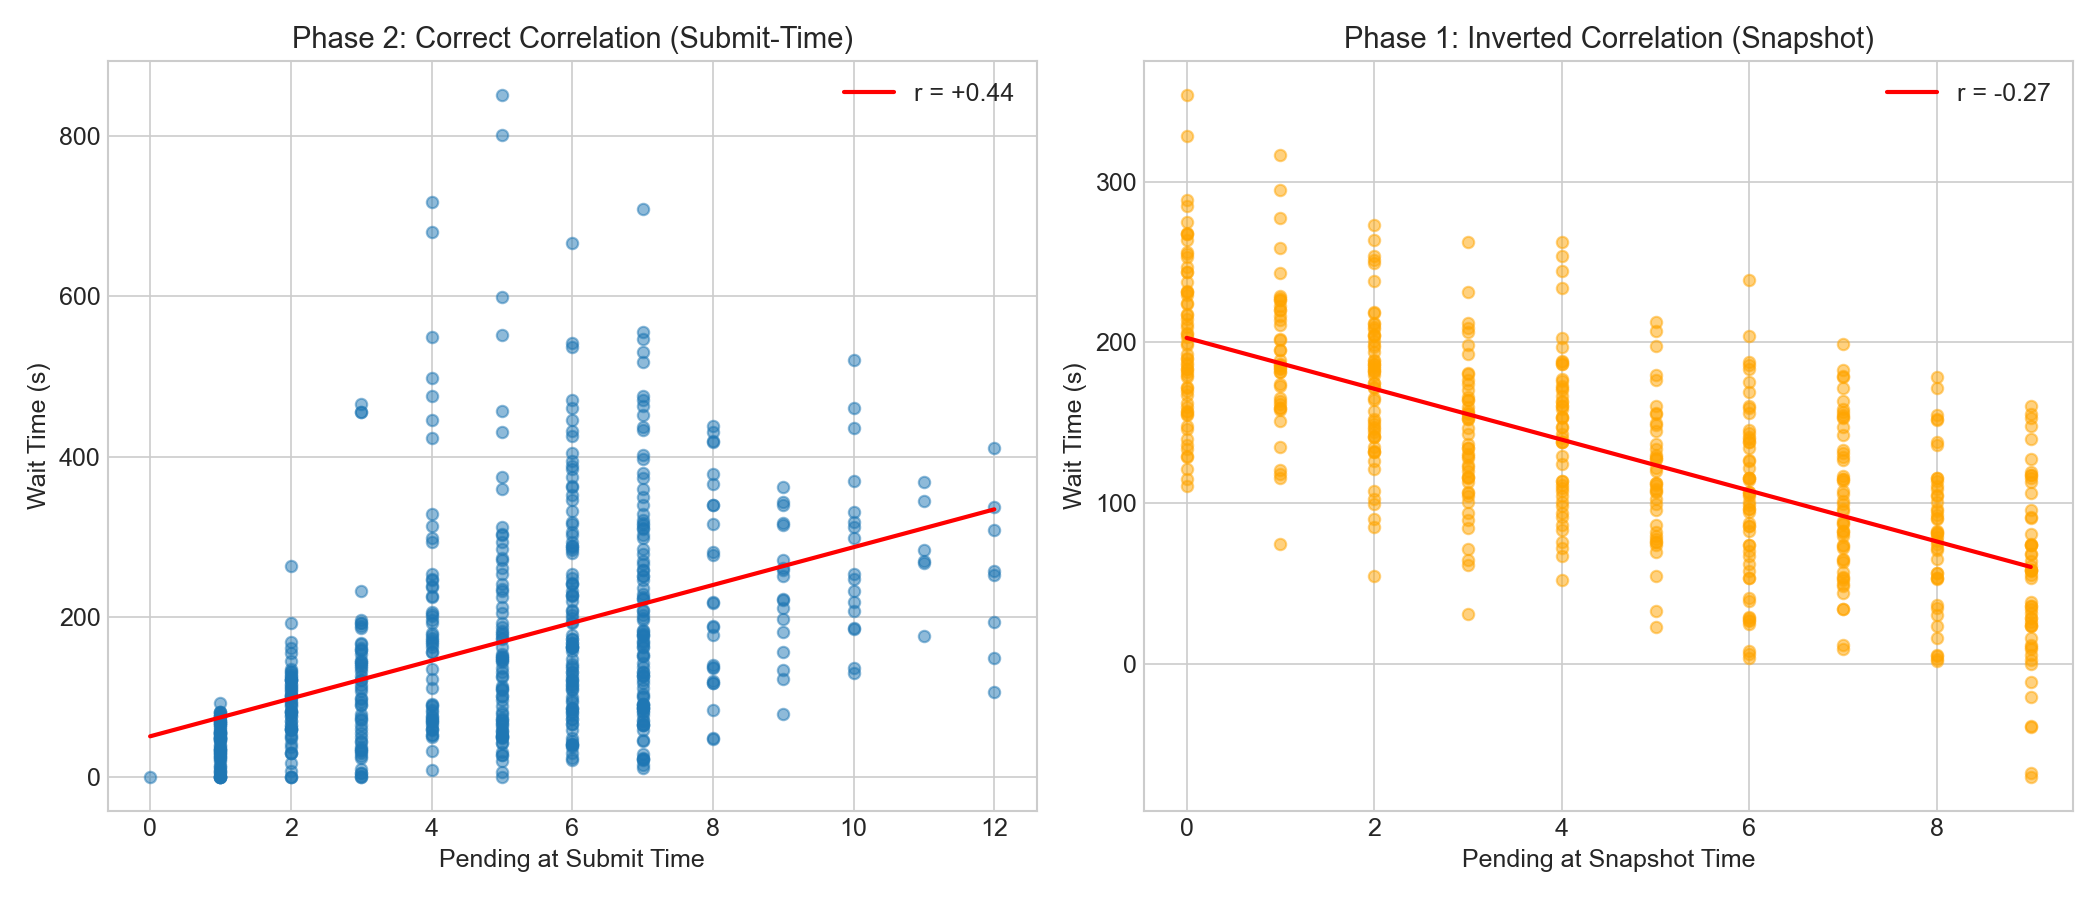
\includegraphics[width=\linewidth]{correlation_comparison.png}
\Description[Two scatterplots of pending count versus wait time]{Two scatterplots side by side. Left panel labelled `Phase 2: Correct Correlation (Submit-Time)' shows pending count at submit time against wait time in seconds, with a positively sloped regression line and r equals plus 0.44. Right panel labelled `Phase 1: Inverted Correlation (Snapshot)' shows pending count at snapshot time against wait time with a negatively sloped regression line and r equals minus 0.27.}
\caption{Submit-time capture corrects the inverted feature correlation. Left: pending count at submit time is positively correlated with realised wait (Pearson $r=+0.44$). Right: the same feature computed from periodic 30\,s snapshots is \emph{anti}-correlated ($r=-0.27$), inverting the causal direction. Submit-time capture is therefore a prerequisite for any downstream decision rule built on queue features.}
\label{fig:correlation}
\end{figure}

A model trained on snapshot-timed features would invert its recommendations: suggesting submission during high congestion and warning during low congestion. Submit-time capture is part of the VGAC instrumentation contract.

\section{Experimental Validation}
\label{sec:validation}

\subsection{Dataset}
Our EKS GPU cluster dataset contains 650 job-lifecycle records (582 usable after de-duplication) collected from an Amazon EKS cluster running on T4 and A10G GPUs. We validate the framework at two instrumentation levels to demonstrate that the tier system accommodates the full spectrum of deployment maturity.

\textbf{Floor (2 features).} Pending and running jobs at submit time, captured per~\S\ref{sec:submit-time}---the minimum viable predictor when no resource instrumentation is available.
\textbf{Ceiling (17+\,features).} The full VGAC feature set: job attributes (CPU, memory, GPU, disk, RDMA, scheduling constraints), cluster state (pending ratio, node pressure, capacity), temporal features, and interaction terms. The ceiling model is trained on 11,982 K8s+Slurm events~\cite{espira2026benchmark}.

\subsection{Floor Model Performance (2 Features)}
For binary classification (long wait $> 120$\,s, base rate 54.1\%) using only \texttt{pending\_at\_submit} and \texttt{running\_at\_submit}, Table~\ref{tab:floor} reports discrimination and calibration.

\begin{table}[t]
\centering
\caption{Binary classification under the 2-feature floor: discrimination and calibration.}
\label{tab:floor}
\small
\begin{tabular}{@{}lrl@{}}
\toprule
\textbf{Metric}    & \textbf{Value} & \textbf{Tier implication} \\
\midrule
AUROC              & 0.756 & Adequate ranking \\
ECE                & 0.077 & Qualifies Tiers 1--2 \\
Precision          & 0.743 & --- \\
Recall             & 0.732 & --- \\
F1                 & 0.738 & --- \\
\bottomrule
\end{tabular}
\end{table}

\subsection{Tier Qualification Assessment}
This is the paper's central result. With ECE $=0.077$, Tier~1 (Annotate) is qualified ($\text{ECE}\le 0.10$); Tier~2 (Warn) is marginal (exceeds 0.07 by 0.007); Tiers~3--4 are not qualified. This honest assessment is invisible to AUROC-only evaluation: a system reporting AUROC $=0.756$ might be deployed with gating enabled, but the ECE analysis reveals this would be premature. Mid-range probabilities (0.35--0.52) show predicted-vs-actual gaps as large as 0.188---exactly the band where Suggest and Gate decisions are most consequential.

\subsection{Floor to Ceiling: Feature Enrichment Unlocks Tiers}
The graduated framework is designed to accommodate the full spectrum of instrumentation maturity. Table~\ref{tab:ceiling} shows the tier progression from the 2-feature floor to the 17+\,feature production VGAC deployment.

\begin{table}[t]
\centering
\caption{Tier qualification progression from floor to ceiling.}
\label{tab:ceiling}
\small
\begin{tabular}{@{}lrrll@{}}
\toprule
\textbf{Configuration}      & \textbf{AUROC} & \textbf{ECE}   & \textbf{Tiers} & \textbf{Features} \\
\midrule
Floor (2 features)          & 0.756          & 0.077          & 1--2           & 2     \\
Production VGAC (17+)       & 0.969          & 0.005          & 1--4           & 17+   \\
\bottomrule
\end{tabular}
\end{table}

\begin{figure}[t]
\centering
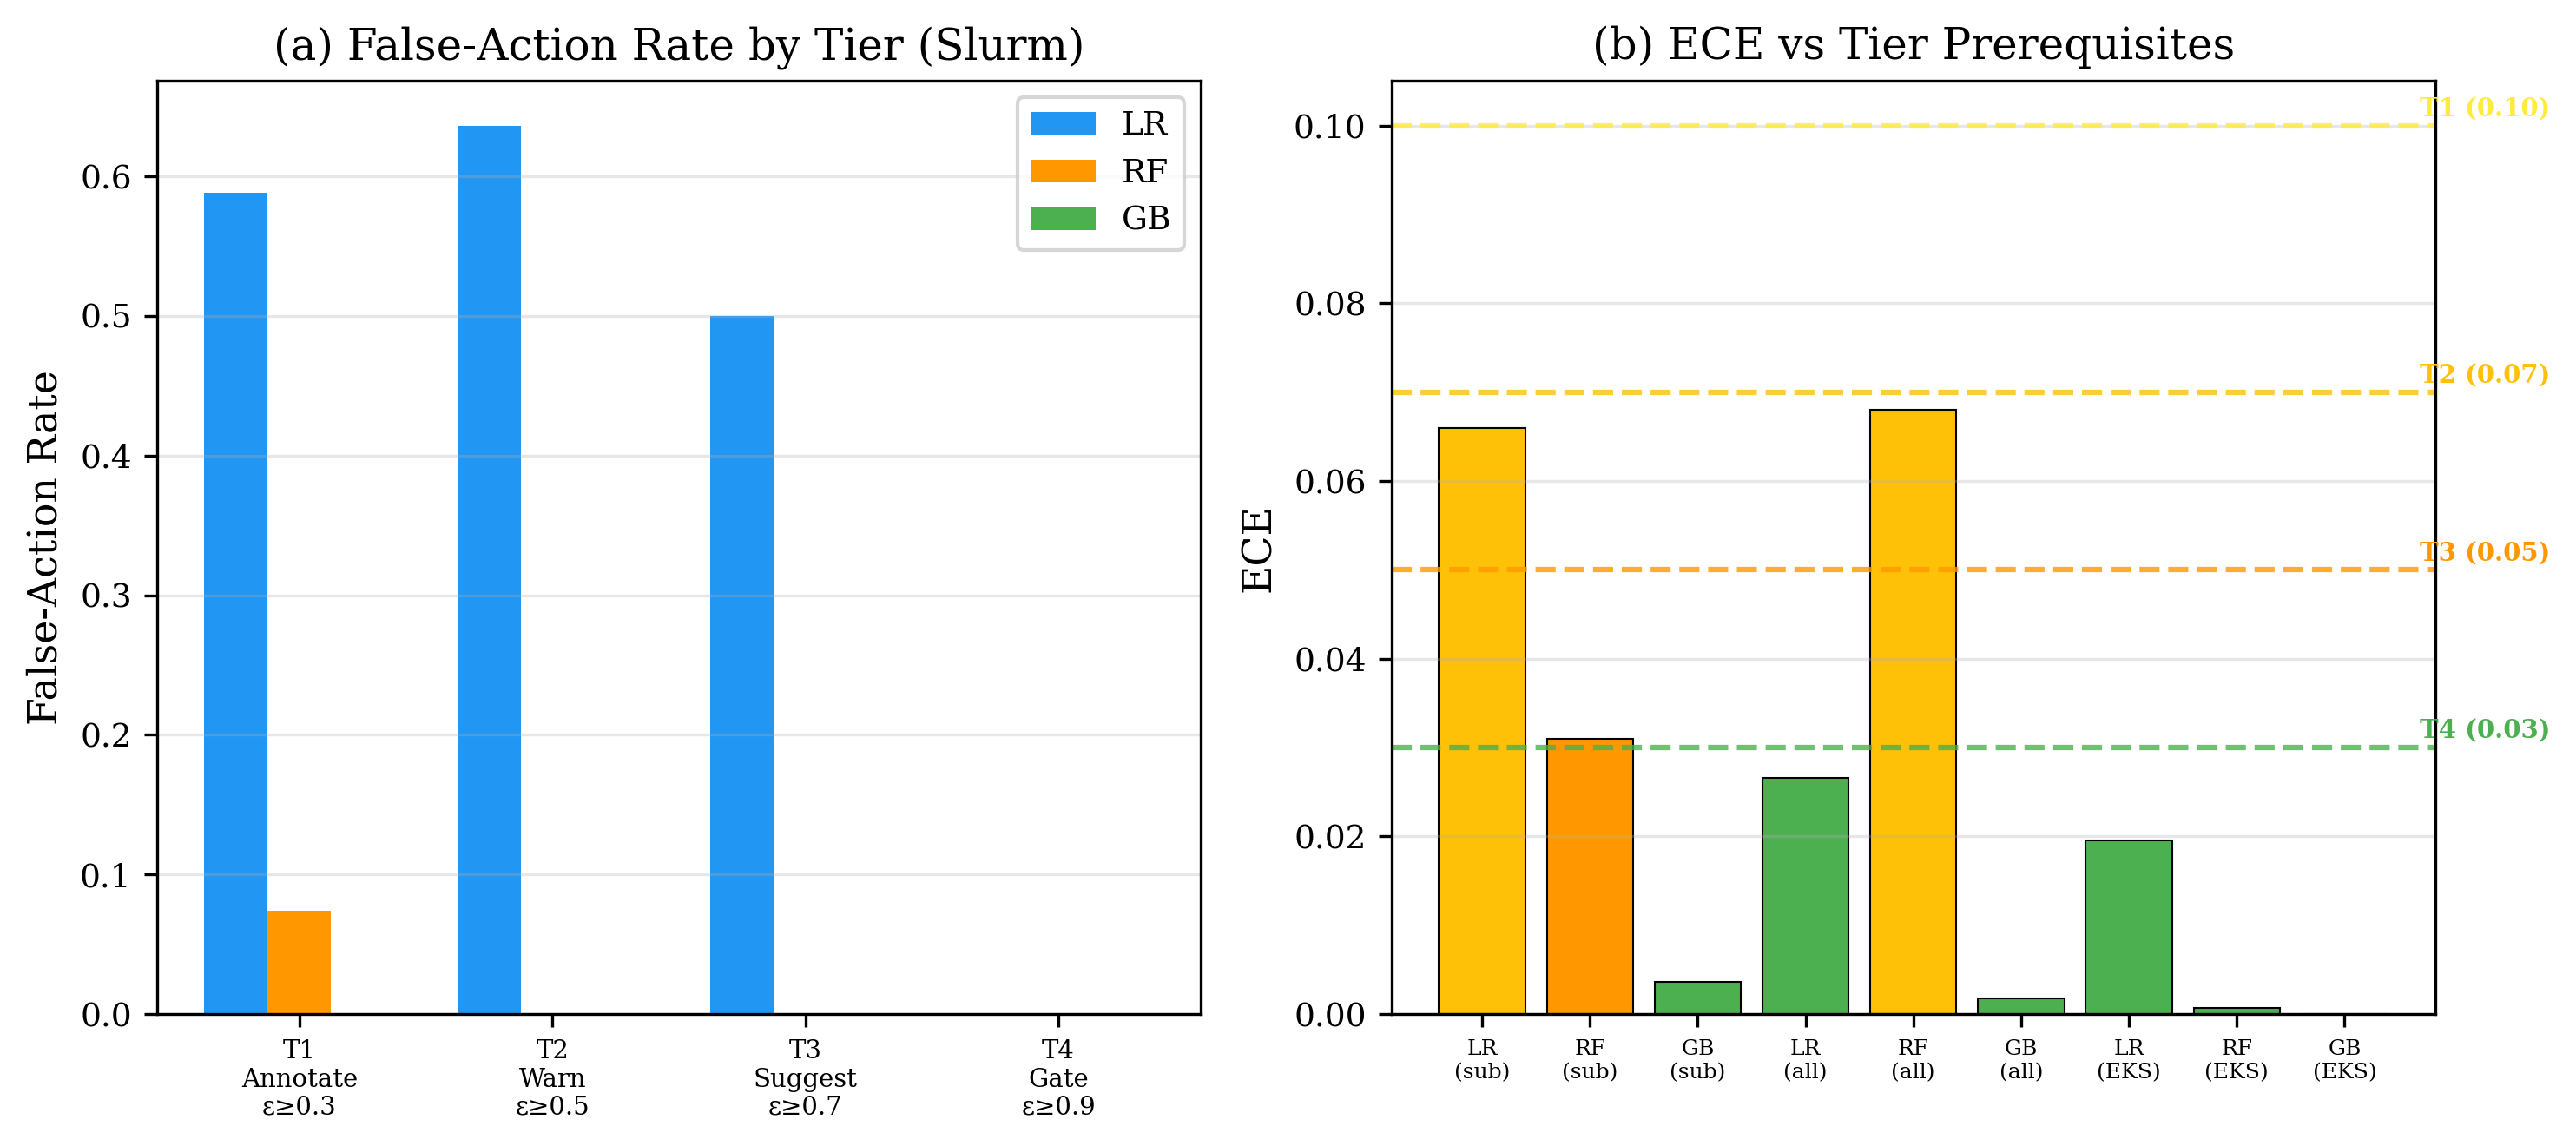
\includegraphics[width=\linewidth]{tier_qualification.png}
\Description[Two bar charts: false-action rate by tier and ECE versus tier prerequisites]{Two-panel bar chart. Panel (a) shows false-action rate by tier on Slurm for three models: logistic regression has rates around 0.59, 0.64, and 0.50 for tiers 1 through 3 with no qualification for tier 4; random forest qualifies for tier 1 only at around 0.07; gradient boosting qualifies for all four tiers with rates near zero. Panel (b) shows ECE bars for the three models across submit-only, all-features, and EKS feature sets, with horizontal dashed reference lines at 0.10, 0.07, 0.05, and 0.03 marking the four tier prerequisites. Only bars below a given dashed line are permitted at that tier.}
\caption{Tier qualification across models and feature sets on a wider benchmark that contextualises Table~\ref{tab:ceiling}. (a) False-action rate per tier on the companion Slurm trace: LR mis-qualifies through Tier~3 while GB clears every threshold. (b) ECE versus the four prerequisites (dashed lines at $0.10/0.07/0.05/0.03$ for T1--T4); only the bars that fall below a given dashed line are permitted at that tier. The pattern generalises the EKS floor-vs-ceiling result: model family \emph{and} feature set jointly determine which tiers are earned.}
\label{fig:tiers}
\end{figure}

With 17+ features and isotonic post-hoc calibration, the production VGAC model reaches ECE $=0.005$---well below the Gate prerequisite of 0.03---qualifying for all four tiers. The $12.7\times$ ECE improvement (0.077 $\to$ 0.005, Fig.~\ref{fig:tiers}b) creates a concrete upgrade path: each instrumentation investment translates into unlocked policy capabilities.

\section{Integration Reference Implementations}
\label{sec:integration}
Both reference integrations enforce tier qualification \emph{at serve time} rather than only at deployment time, so degraded models automatically reduce their action scope. \textbf{Kubernetes:} a mutating admission webhook intercepts Pod creation, queries the prediction service ($<10$\,ms), and annotates the Pod with the predicted probability and qualified tier; a model whose rolling ECE drifts above $0.05$ silently stops emitting Suggest and Gate annotations until recalibration restores qualification. \textbf{Slurm:} a \texttt{job\_submit} plugin attaches tier-qualified predictions to the job's \texttt{Comment} field, surfacing Warn-level alerts via \texttt{slurm\_info} when probability and tier jointly warrant notification. Both follow the same loop: \texttt{prob = predict(features); tier = get\_qualified\_tier(prob, current\_ece); annotate(job, prob, tier)}---evaluated per request against the model's rolling ECE, so graceful degradation is dynamic, not a build-time decision.

\section{Discussion}
The floor-to-ceiling validation (Table~\ref{tab:ceiling}, Fig.~\ref{fig:tiers}) shows the framework accommodates the full instrumentation spectrum: minimal submit-time signal closes the reactive gap for advisory tiers, while 17+ features support autonomous admission gating (ECE $0.005 \ll 0.03$). Without calibration prerequisites a team deploying the 2-feature model at AUROC $0.756$ might enable gating; the framework prevents this by requiring each tier to be \emph{earned} through demonstrated ECE.
\paragraph{Limitations.} The ECE prerequisites in Table~\ref{tab:tiers} are informed by operational intuition; formal cost-sensitive analysis could tighten them per operator. The 2-feature validation uses one EKS cluster ($n=650$); cross-cluster evaluation across heterogeneous schedulers is the subject of a companion benchmark~\cite{espira2026benchmark}.

\section{Related Work}
Decima~\cite{decima} learns scheduling policies via reinforcement learning but does not address calibration or user-facing decision rules. Borg~\cite{borg} and Firmament~\cite{firmament} optimize placement; our focus is the prediction-to-decision interface at submit time. Elkan~\cite{elkan2001} formalizes cost-sensitive classification, in which the optimal threshold depends on cost ratios; we extend this idea to graduated actions where each tier has a different cost profile and a different calibration requirement. Guo et al.~\cite{guo2017calibration} established ECE as a standard calibration metric; we operationalize ECE as a gate that constrains permissible actions.

\section{Conclusion}
VGAC is a full-stack GPU cluster observability platform whose predictive intelligence is calibration-gated: calibration quality determines permissible action severity, and each tier of intervention must be \emph{earned} through demonstrated ECE. The 2-feature floor (ECE $0.077$) honestly qualifies only for annotation; the 17+\,feature production VGAC model (ECE $0.005$) qualifies for all four tiers including autonomous gating---a $12.7\times$ improvement invisible to AUROC-only evaluation. Submit-time capture ($r=-0.27 \to +0.44$, Fig.~\ref{fig:correlation}) further shows that correct measurement is a prerequisite for correct decisions. With the companion SLI/SLO framework~\cite{espira2026reliability}, VGAC completes the path from calibrated prediction to safe scheduling policy.

\section*{Disclosure of Generative AI Use}
In accordance with the ACM Policy on Authorship and the Use of Generative
AI Tools, the authors disclose the following: portions of the manuscript
text were edited with the assistance of a large language model (Anthropic
Claude, accessed during 2026) used as a writing aid for clarity, grammar,
and concision on author-drafted content. The model was not used to
generate experimental results, design or run experiments, interpret data,
construct tables, derive equations, or compose citations. All scientific
content---including the calibration framework, tier prerequisites,
submit-time capture methodology, empirical results, tables, and the bibliography---
was conceived, executed, and verified by the human authors, who take full
responsibility for the integrity, originality, and accuracy of the work.

\begin{acks}
We thank Saint Peter's University for support of this work.
\end{acks}

\bibliographystyle{ACM-Reference-Format}
\bibliography{refs}

\end{document}
